%%%%%%%%%%%%%%%%%%%%%%%%%%%%%%%%%%%%%%%%%
% Class Notes Template
% LaTeX Template
% By: Ryan Grove
%%%%%%%%%%%%%%%%%%%%%%%%%%%%%%%%%%%%%%%%%

%----------------------------------------------------------------------------------------
%	PACKAGES AND OTHER DOCUMENT CONFIGURATIONS
%----------------------------------------------------------------------------------------

\documentclass[paper=a4, fontsize=11pt]{scrartcl} % A4 paper and 11pt font size

\usepackage[T1]{fontenc} % Use 8-bit encoding that has 256 glyphs
\usepackage{fourier} % Use the Adobe Utopia font for the document - comment this line to return to the LaTeX default
\usepackage[english]{babel} % English language/hyphenation
\usepackage{amsmath,amsfonts,amsthm} % Math packages

\usepackage{lipsum} % Used for inserting dummy 'Lorem ipsum' text into the template

\usepackage{sectsty} % Allows customizing section commands
\allsectionsfont{\centering \normalfont\scshape} % Make all sections centered, the default font and small caps

\usepackage{fancyhdr} % Custom headers and footers
\pagestyle{fancyplain} % Makes all pages in the document conform to the custom headers and footers
\fancyhead{} % No page header - if you want one, create it in the same way as the footers below
\fancyfoot[L]{} % Empty left footer
\fancyfoot[C]{} % Empty center footer
%\fancyfoot[R]{\thepage} % Page numbering for right footer
\renewcommand{\headrulewidth}{0pt} % Remove header underlines
\renewcommand{\footrulewidth}{0pt} % Remove footer underlines
\setlength{\headheight}{13.6pt} % Customize the height of the header

\numberwithin{equation}{section} % Number equations within sections (i.e. 1.1, 1.2, 2.1, 2.2 instead of 1, 2, 3, 4)
\numberwithin{figure}{section} % Number figures within sections (i.e. 1.1, 1.2, 2.1, 2.2 instead of 1, 2, 3, 4)
\numberwithin{table}{section} % Number tables within sections (i.e. 1.1, 1.2, 2.1, 2.2 instead of 1, 2, 3, 4)

\setlength\parindent{0pt} % Removes all indentation from paragraphs - comment this line for an assignment with lots of text

\usepackage{lastpage}
\usepackage{fancyhdr}
\cfoot{\thepage\ of \pageref{LastPage}}

\def\v{\hbox{$\mathbf v$}}
\def\w{\hbox{$\mathbf w$}}
\def\u{\hbox{$\mathbf u$}}
\def\x{\hbox{$\textbf{x}$}}
\def\z{\hbox{$\mathbf z$}}
\def\a{\hbox{$\mathbf a$}}
\def\b{\hbox{$\mathbf b$}}
\def\L{\hbox{$\mathcal L$}}
\def\C{\hbox{$\mathbb C$}}
\def\B{\hbox{$\mathcal B$}}
\def\R{\hbox{$\mathbb R$}}
\def\X{\hbox{$\underline X$}}
\def\Q{\hbox{$\mathbb Q$}}
\def\R{\hbox{$\mathbb R$}}
\def\N{\hbox{$\mathbb N$}}
\def\C{\hbox{$\mathbb C$}}
\def\0{\hbox{$\mathbf 0$}}
\def\Y{\hbox{$\underline Y$}}
\def\a{\hbox{$\mathbf a$}}
\def\u{\hbox{$\mathbf u$}}
\def\w{\hbox{$\mathbf w$}}
\def\y{\hbox{$\mathbf y$}}
\def\X{\hbox{$\underline X$}}
\def\dd{\hbox{$\partial $}}
\def\B{\hbox{$\mathcal B$}}
\def\F{\hbox{$\mathcal F$}}
\def\L{\hbox{$\mathcal L$}}
\def\M{\hbox{$\mathcal M$}}
\def\D{\hbox{$\mathscr {D}$}}
\def\RR{\hbox{$\mathscr{R}$}}
\def\I{\hbox{$\mathcal I$}}

\usepackage{amssymb}
%\theoremstyle{plain}
\usepackage[margin = .75in]{geometry}
\newtheorem{claim}{Claim}
\newtheorem{theorem}{Theorem}[section]
\newtheorem{lemma}[theorem]{Lemma}
\newtheorem{proposition}[theorem]{Proposition}
\newtheorem{corollary}[theorem]{Corollary}
\newtheorem{problem}[theorem]{Problem}
%\theoremstyle{definition}
\newtheorem{definition}[theorem]{Definition}
%\theoremstyle{remark}
\newtheorem{remark}[theorem]{Remark}
\newtheorem{remarks}[theorem]{Remarks}
\newtheorem{example}[theorem]{Example}
\newcommand{\ds}{\displaystyle}
\newcommand{\ZZ}{\mathbb{Z}}
\newcommand{\QQ}{\mathbb{Q}}
\newcommand{\e}{\varepsilon}
\newcommand{\bbf}{\textbf}
\newcommand{\p}{\parallel}
\usepackage{color}
\newcommand{\field}[1]{\mathbb{#1}}
\usepackage{amsmath}
\usepackage{amsthm}
\usepackage{amssymb}
\usepackage{mathrsfs}
\usepackage{cancel}
\usepackage{upgreek}
\usepackage{graphicx}
\usepackage{multirow}
\usepackage{setspace}
\usepackage{url}
\usepackage{subfigure}
\usepackage{enumerate}
\usepackage{cases}
\usepackage{mathrsfs}
\usepackage{rotating}

%----------------------------------------------------------------------------------------
%	TITLE SECTION
%----------------------------------------------------------------------------------------

\newcommand{\horrule}[1]{\rule{\linewidth}{#1}} % Create horizontal rule command with 1 argument of height

\title{	
\normalfont \normalsize 
\textsc{Ryan Grove, Clemson University, MATH1080 - 9} \\ [25pt] % Your name, university, class
\horrule{0.5pt} \\[0.4cm] % Thin top horizontal rule
\huge Section 7.8: Improper Integrals \\ % The assignment title
\horrule{2pt} \\[0.5cm] % Thick bottom horizontal rule
}

\author{Date:} % The due date

\date{\normalsize February 10, 2016} % A custom date

\begin{document}

\maketitle % Print the title

\begin{flushleft}
\begin{tabular}{l l}
Name: \rule{3.2in}{.01cm}  & {}%Table number: \rule{1in}{.01cm}\\
\end{tabular}
\end{flushleft}

%----------------------------------------------------------------------------------------
%	Lecture
%----------------------------------------------------------------------------------------

\section*{\textbf{Lecture:}}

In defining a definite integrals $\ds\int_a^b f(x)dx$ we dealt with a function $f$ defined on a finite interval $[a,b]$ and we assumed that $f$ does not have an infinite discontinuity. In this section we extend the concept of the definite integral to the case where the interval is infinite and also to the case where $f$ has an infinite discontinuity in $[a,b]$. In either case the integral is called an \underline{\hspace{1.25in}} integral.\\

\section*{Type 1: Infinite Intervals}
Consider the infinite region $S$ that lies under the curve $y=\ds\frac{1}{x^2}$, above the $x-$axis, and to the right of the line $x=1$.

\[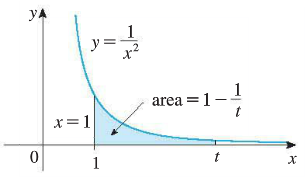
\includegraphics[scale=0.6]{7-8pic1.png}\]

You might think that, since $S$ is infinite in extent, its area must be infinite, but let's take a closer look. The area of the part of $S$ that lies to the left of the vertical line $x=t$ (shaded above) is:\\

\[A(t) = \hspace{3in}\]
\indent

Notice that $A(t)<1$ no matter how large $t$ is chosen. We also observe that:

\[\ds\lim_{t\to\infty} A(t) = \hspace{2in}\]
\indent

Thus the area of the shaded region approaches \underline{\hspace{0.3in}} as $t\to\infty$, so we say that the area of the infinite region $S$ is equal to \underline{\hspace{0.3in}} and we write:\\

\[\ds\int_1^{\infty} \ds\frac{1}{x^2}dx = \hspace{2.5in}\]
\indent

Using this example as a guide, we define the integral of $f$ (not necessarily a positive function) over an \textbf{infinite} interval as the \underline{\hspace{1in}} of integrals over \textbf{finite} intervals.\\
\indent

\[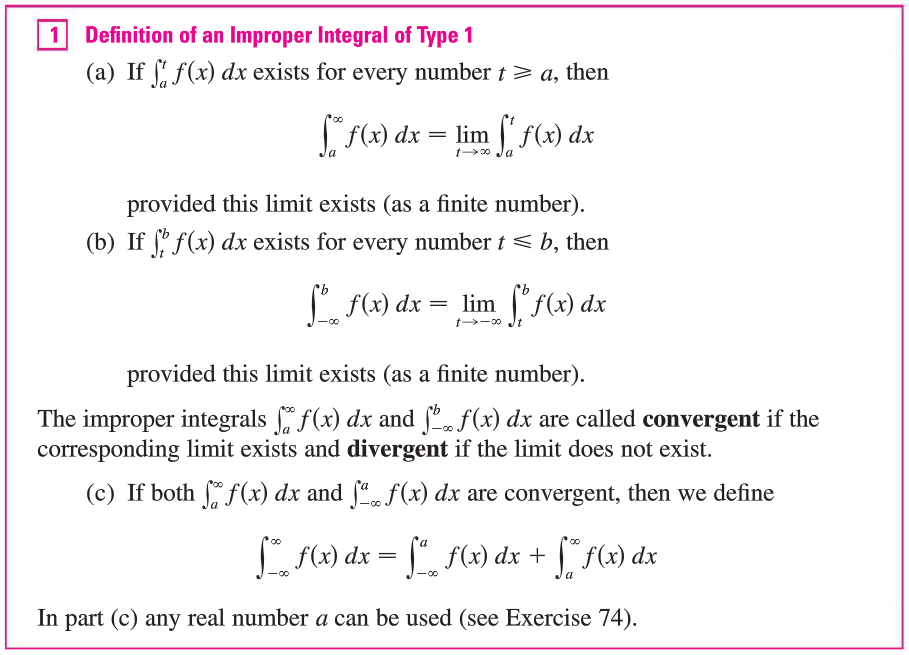
\includegraphics[scale=0.45]{7-8pic2.png}\]
\indent

\underline{Example 1}: Determine whether the integral $\ds\int_1^\infty \ds\frac{1}{x}\text{ }dx$ is convergent or divergent.\\
\indent

\vspace{3in}

\newpage

Let's compare the result of Example 1 with the example given at the beginning of this section:

\[\ds\int_1^{\infty}\ds\frac{1}{x^2}\text{ }dx \text{  converges }  \hspace{1in}  \ds\int_1^{\infty}\ds\frac{1}{x}\text{ }dx \text{  diverges }\]
\indent

Geometrically, this says that although the curves $y=\ds\frac{1}{x^2}$ and $y=\ds\frac{1}{x}$ look very similar for $x>0$, the region under $y=\ds\frac{1}{x^2}$ to the right of $x=1$ has finite area whereas the corresponding region under $y=\ds\frac{1}{x}$ has infinite area. Note that both $\ds\frac{1}{x^2}$ and $\ds\frac{1}{x}$ approach 0 as $x\to\infty$, but $\ds\frac{1}{x^2}$ approaches 0 faster than $\ds\frac{1}{x}$. The values of $\ds\frac{1}{x}$ don't decrease fast enough for its integral to have a finite value.\\

\[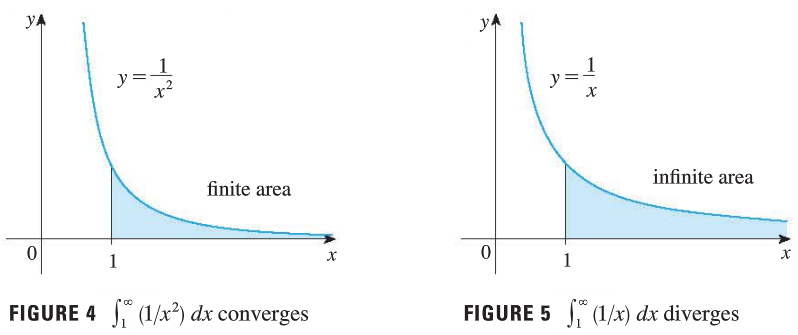
\includegraphics[scale=0.45]{7-8pic3.png}\]
\indent

\underline{Example 2}: Evaluate $\ds\int_{-\infty}^0 xe^x \text{ }dx$.\\
\indent

\vspace{3.5in}

\newpage

\underline{Example 3}: Evaluate $\ds\int_{-\infty}^\infty \ds\frac{1}{1+x^2}\text{ }dx$.\\
\indent

\vspace{7in}

Since $\ds\frac{1}{1+x^2}>0$, the given improper integral can be interpreted as the \underline{\hspace{0.75in}} of the infinite region that lies under the curve $y=\ds\frac{1}{1+x^2}$ and above the $x-$axis.
\[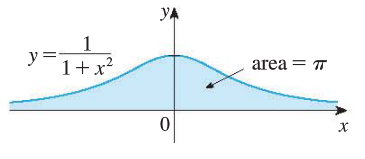
\includegraphics[scale=0.5]{7-8pic4.png}\]


\newpage

\underline{Example 4}: For what values of $p$ is the integral
\[\ds\int_1^{\infty}\ds\frac{1}{x^p}\text{ }dx\]
covergent?\\
\indent

\textbf{SOLUTION:} We know from Example 1 that if $p=1$, then the integral is divergent, so let's assume that $p\neq 1$. Then,\\

\vspace{6.4in}

In summary:\\
\indent\\

\fbox{
  \parbox{\textwidth}{
  \vspace{5pt}
  \[\quad \ds\int_1^{\infty}\ds\frac{1}{x^p} \text{ is \underline{\hspace{1.25in}} if } p>1 \text{ and \underline{\hspace{1.25in}} if } p\leq 1. \quad\]
}}

\newpage

\section*{Type 2: Dicontinuous Integrands}
Suppose that $f$ is a positive continuous function defined on a finite interval $[a,b)$ but has a vertical asymptote at $b$. Let $S$ be the unbounded region under the graph of $f$ and above the $x-$axis between $a$ and $b$.\\

\[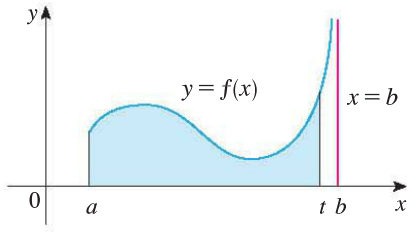
\includegraphics[scale=0.4]{7-8pic5.png}\]

\textbf{Note}:\\
\quad $\bullet$ For Type 1 integrals (Infinite Intervals),\\
\hspace{1.5in} the region is extended indefinitely in a \underline{\hspace{1.5in}} direction.\\
\indent

\quad $\bullet$ For Type 2 integrals (Discontinuous Integrands),\\
\hspace{1.5in} the region is infinite in a \underline{\hspace{1.25in}} direction.\\
\indent
\indent

The area here of the part of $S$ between $a$ and $t$ (shaded above) is:\\
\[ A(t) = \ds\int_a^t f(x)\text{ }dx.\]\\
\indent

If it happens that $A(t)$ approaches a definite number $A$ as $t\to{b^-}$, then we say that the area of the region $S$ is $A$ and we write:

\[\ds\int_a^b f(x)\text{ }dx = \hspace{2in}\]
\indent\\
\indent\\
\indent

We use this equation to define an improper integral of Type 2 even when $f$ is not a positive function, no matter what type of discontinuity $f$ has at $b$.\\
\indent

\[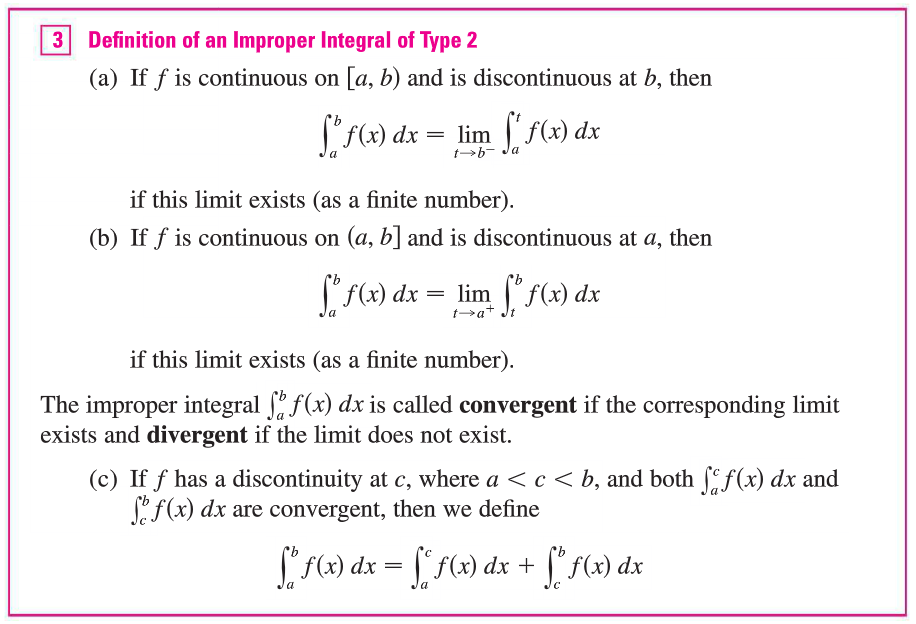
\includegraphics[scale=0.5]{7-8pic6.png}\]
\indent\\
\indent

\[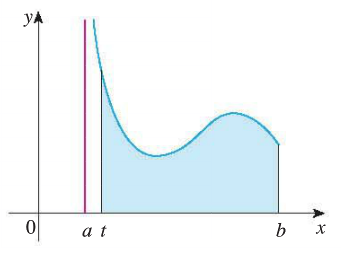
\includegraphics[scale=0.5]{7-8pic7.png} \quad \quad 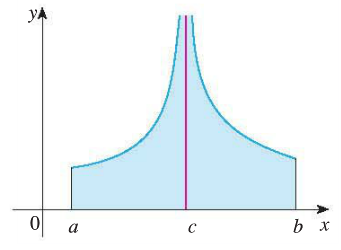
\includegraphics[scale=0.5]{7-8pic8.png}\]
\indent

\newpage
\underline{Example 5}: Find $\ds\int_2^5\ds\frac{1}{\sqrt{x-2}}\text{ }dx$.\\
\indent

\vspace{3.45in}

*Thus the given improper integral is \underline{\hspace{1.25in}} and, since the integrand is positive, we can interpret the value of the integral as the area of the shaded region:\\
\vspace{-10pt}
\hspace{5in}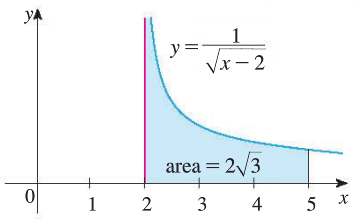
\includegraphics[scale=0.4]{7-8pic9.png}

\underline{Example 6}: Determine whether $\ds\int_0^{\pi/2}\sec x \text{ }dx$ converges or diverges.\\


\vspace{3.4in}

*Thus the given improper integral is \underline{\hspace{1.25in}}.\\

\newpage
\underline{Example 7}: Evaluate $\ds\int_0^3\ds\frac{dx}{x-1}\text{ }dx$ if possible.\\
\indent

\vspace{6.6in}

\textbf{*WARNING:} If we had not noticed the asymptote $x=1$ in Example 7 and had instead confused the integral with an ordinary integral, then we might have made the following erroneous calculation:
\[\ds\int_0^3\ds\frac{dx}{x-1} = \ln|x-1|\bigg{]}_0^3 = \ln 2 - \ln 1 = \ln 2.\]

This is WRONG because the integrand is improper and MUST be calculated in terms of \underline{\hspace{1in}}. \textbf{FROM NOW ON}, whenever you meet the symbol $\ds\int_a^b f(x)\text{ }dx$ you must decide, by looking at the function $f$ on the interval $[a,b]$, whether it is an ordinary definite integral or an improper integral.\\
\indent

\newpage

\underline{Example 8}: Evaluate $\ds\int_0^1 \ln x \text{ }dx$.\\
\indent

\newpage
\section*{A Comparison Test for Improper Integrals}
Sometimes it is impossible to find the exact value of an improper integral and yet it is important to know whether it is convergent or divergent. In such cases the following theorem is useful. Although we state it for Type 1 integrals, a similar theorem is also true for Type 2 integrals.

\[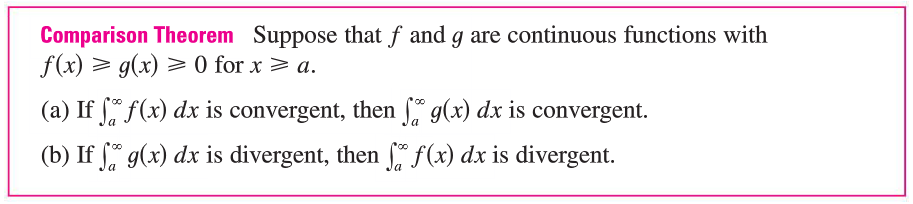
\includegraphics[scale=0.5]{7-8pic10.png}\]

We omit the proof of the Comparison Theorem, but the illustration shown below makes it seem plausible. If the area under the top curve $y=f(x)$ is finite, then so is the area under the bottom curve $y=g(x)$. And if the area under $g(x)$ is infinite, then so is the area under $y=f(x)$. \\
\indent\\
\indent


\[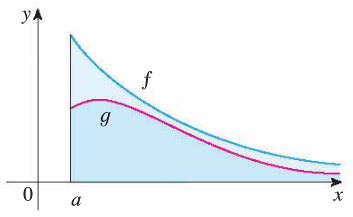
\includegraphics[scale=0.5]{7-8pic11.png}\]
\indent\\
\indent

Note that the reverse is not necessarily true: \\
\indent

\quad \quad $\bullet$ If $\ds\int_a^\infty g(x)\text{ }dx$ is convergent, $\ds\int_a^\infty f(x)\text{ }dx$ may or may not be convergent, and\\
\indent

\quad \quad $\bullet$ If $\ds\int_a^\infty f(x) \text{ }dx$ is divergent, $\ds\int_a^\infty g(x)\text{ }dx$ may or may not be divergent.\\


\newpage
\underline{Example 9}: Show that $\ds\int_0^\infty e^{-x^2}\text{ }dx$ is convergent.\\
\indent


\vspace{5.5in}
\[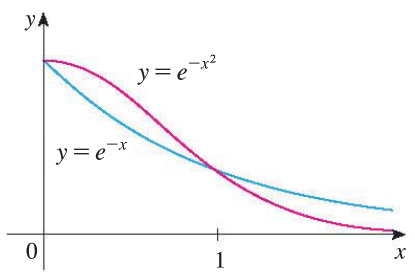
\includegraphics[scale=0.4]{7-8pic12.png}\]

\indent\\
\indent

\underline{Example 10}: The integral $\ds\int_1^{\infty} \ds\frac{1+e^{-x}}{x}\text{ }dx$ is divergent by the Comparison Theorem because
\[\ds\frac{1+e^{-x}}{x} > \ds\frac{1}{x}\]
and $\ds\int_1^{\infty}\ds\frac{1}{x}\text{ }dx$ is divergent by Example 1.\\



%\fbox{
%  \parbox{\textwidth}{
%  \vspace{5pt}

















%----------------------------------------------------------------------------------------

\end{document}